\section{Linear Map}
\subsection{The Vector Space of Linear Maps}
  \paragraph{1.}
  \begin{proof}
    If $T$ is linear, then $T(0,0,0)=0$ and therefore $b=0$. Meanwhile, 
    $T(2,2,2)=2T(1,1,1)$ implies $12+8c=12+2c$. Hence, $c=0$. The proof of the 
    converse part is trivial.
  \end{proof}

  \paragraph{3.}
  \begin{proof}
    Let $e_i$ be the $i$-th vector in the standard base of $\mathbb{F}^n$ and 
    suppose that $Te_i = \sum_{j=1}^n A_{1,j}e_j$. Then for $x=(x_1,\dots,x_n)^T 
    \in\mathbb{F}^n$,
    \[
      Tx = T\left(\sum_{i=1}^n x_ie_i\right) = \sum_{i=1}^n x_iTe_i =
      \sum_{i=1}^n x_i\sum_{j=1}^nA_{j,i}e_j = 
      \sum_{j=1}^n\left(\sum_{i=1}^nA_{j,i}x_i\right) e_j.
    \]
  \end{proof}

  \paragraph{5.}
  \begin{proof}
    Too lengthy to write it down...
  \end{proof}

  \paragraph{7.}
  \begin{proof}
    Let $\{x_0\}$ be a basis of $V$ and $\lambda$ be a scalar such that $Tx_0=
    \lambda x_0$. By the linearity of $T$, for every $x=kx_0$ in $V$, $Tx=kTx_0
    =k\lambda x_0=\lambda(kx_0)=\lambda x$.
  \end{proof}

  \paragraph{9.}
  \begin{solution}
    From the additivity condition we can derive that $\varphi(kz)=k\varphi(z)$
    for any $k\in\mathbb{Q}$. Hence we can try some functions where $\varphi(iz)
    =i\varphi(z)$ fails. It turns out that $\varphi(z)=\Im(z)$ is one of the 
    maps required.
  \end{solution}

  \paragraph{11.}
  \begin{proof}
    Let $\{\alpha_1,\dots,\alpha_p\}$ and $\{\alpha_1,\dots,\alpha_p,\beta_1,
    \dots,\beta_q\}$ be bases of $U$ and $V$ respectively. Then the linear map 
    which maps $\alpha_i$ to $T\alpha_i$ and maps $\beta$ to $0$. Clear that
    it is the desired linear map. 
  \end{proof}

  \paragraph{13.}
  \begin{proof}
    Suppose that $v_k$ is in the span of the other vectors and let $w_i=0$ for 
    each $i\ne k$ and $w_k\ne 0$. No $T\in\mathcal{L}(V, W)$ can maps $v_i$ to 
    $w_i$ since the linearity of $T$ would force $w_k$ to be $0$, leading to a 
    contradiction.
  \end{proof}

% end

\subsection{Null Spaces and Ranges}
  \paragraph{2.}
  \begin{proof}
    Since $S$ maps every vector of $V$ into the null space of $T$, the map $TS$
    is the zero map. Hence $(ST)^2 = S(TS)T = 0$.
  \end{proof}

  \paragraph{4.}
  \begin{proof}
    Suppose $S,T\in\mathcal{L}(\mathbb{R}^5,\mathbb{R}^4)$ maps and only maps 
    $e_1,e_2,e_3$ and $e_3,e_4,e_5$ to the zero vector respectively. Then $e_1,
    e_2,e_4,e_5\notin\nul(S+T)$, implying that $\dim\nul(S+T)<2$. Hence $\{T\in
    \mathcal{L}(\mathbb{R}^5,\mathbb{R}^4\,:\,\dim\nul T>2)\}$ is not a subspace
    of $\mathcal{L}(\mathbb{R}^5,\mathbb{R}^4)$.
  \end{proof}

  \paragraph{6.}
  \begin{proof}
    It follows immediately from the rank-nullity theorem and the fact that $\dim
    \nul T$ and $\dim\range T$ are integers.
  \end{proof}

  \paragraph{8.}
  \begin{proof}
    Let $\{w_1,\dots,w_m\}$ be a basis of $W$ and $S,T\in\mathcal{L}(V,W)$ be 
    two linear maps such that $\range S=\spn(w_1)$ and $\range T=\spn(w_2,\dots,
    w_n)$. Clear that $\range(S+T)=W$. Hence, the set described is not a 
    subspace of $\mathcal{L}(V,W)$.
  \end{proof}

  \paragraph{10.}
  \begin{proof}
    For every $y\in\range T$ there exists some $x=\sum x_iv_i\in V$ such that 
    \[
      y=Ty = T\left(\sum_{i=1}^n x_iv_i\right) = \sum_{i=1}^n x_iTv_i.
    \]
    Hence, $\range T=\spn(Tv_1,\dots,Tv_n)$.
  \end{proof}

  \paragraph{12.}
    For readers who familiar with the orbit-stabilizer theorem or just the 
    (group) homomorphism, the proof should be straightforward.
  \begin{proof}
    For every nonzero $y$ in $\range T$, there exists some $x\in V$ such that 
    $Tx=y$. For each $y\ne 0$, we choose one such $x$, put them all together and 
    put $0$ into them to get $U$. By the construction, clear that $T(U) = 
    \range T$ and , $U\cap\nul T=\{0\}$.
  \end{proof}

  \paragraph{14.}
  \begin{proof}
   By the rank-nullity theorem, 
   \[
     \dim\nul T + \dim\range T = 8 \quad\Rightarrow\quad
     \dim\range T = 5 = \dim\mathbb{R}^5.
   \]
   Hence, $\range T = \mathbb{R}^5$ and therefore $T$ is surjective.
  \end{proof}

  \paragraph{16.}
    Actually, the cosets of the kernel partition the whole space.
  \begin{proof}
    Let $\{v_1,\dots,v_n\}$ be a basis of $\range T$ and $Tu_i=v_i$ for $i=1,2,
    \dots,n$. Denote $\spn(u_1,\dots,u_n)$ by $U$. We now prove that $V=U+\nul
    T$. For every $x\in V$, suppose that $Tx=y=\sum y_iv_i$ and $\tilde{x}=\sum
    y_iu_i$. Note that $\tilde{x}\in U$ and $T(x-\tilde{x})=Tx-T\tilde{x}=0$, 
    i.e., $x-\tilde{x}\in\nul T$. Hence, $V=U+\nul T$. As both of $U$ and $\nul
    T$ are finite-dimensional, so is $V$.
  \end{proof}

  \paragraph{18.}
  \begin{proof}
    By the rank-nullity theorem, clear that $\dim V \ge \dim\range T =\dim W$ if
    there exists some surjective $T\in\mathcal{L}(V,W)$. \par
    Assume that $\dim V\ge\dim W$ and let $\{v_1,\dots,v_n\}$ and $\{w_1,\dots,
    w_m\}$ be bases of $V$ and $W$ respectively. Then the linear map which
    maps $v_i$ to $w_i$ for each $1\le i\le m$ is surjective.
  \end{proof}

  \paragraph{20.}
  \begin{proof}
    If $T$ is injective, then for every $y\in\range T$, there exists exactly 
    one $x\in V$ such that $y=Tx$. Let $S$ be the map which maps $y$ to such
    $x$. It is linear since for every $y_1,y_2\in\range T$ and scalar $a,b$,
    supposing $Sy_i = x_i$,
    \[
      T(ax_1+bx_2) = aTx_1 + bTx_2 = ay_1 + by_2.
    \]
    implying $S(ay_1+by_2) = ax_1+bx_2 = aSy_1 + bSy_2$. For every $x\in V$,
    $(ST)x = S(Tx) = x$. \par
    Suppose there exists some $S\in \mathcal{L}(W,V)$ such that $ST=I$. Then
    \[
      Tx_1 = Tx_2 \quad\Rightarrow\quad
      STx_1 = STx_2 \quad\Rightarrow\quad
      x_1 = x_2.
    \]
    Hence, $T$ is injective.
  \end{proof}

  \paragraph{22.}
  \begin{proof}
    Let $\tilde{T}$ be the restriction of $T$ to $\nul ST$. It is still a linear
    map since $\nul ST$ is a subspace of $U$. Note that $x\in\nul ST$ iff $(ST)x
    =0$ iff $Tx\in\nul S$. Hence, $\range\tilde{T}\subset\nul S$. Thus, by the 
    rank-nullity theorem,
    \[
      \dim\range\tilde{T} \le \dim\nul S \quad\Rightarrow\quad
      \dim\nul ST - \dim\nul\tilde{T} \le \dim\nul S.
    \]
    Since $\nul\tilde{T} \le \nul T$, this implies $\dim\nul ST \le \dim\nul S +
    \dim\nul T$.
  \end{proof}

  \paragraph{24.}
  \begin{proof}
    If there exists $S\in\mathcal{L}(W,W)$ such that $T_2=ST_1$, then $\nul T_2
    =\nul ST_1$. Hence for every $x\in\nul T_1$, as $S(T_1x)=S0 = 0$, $x\in\nul
    T_2$. Therefore, $\nul T_1\subset\nul T_2$.\par
    Now we suppose $\nul T_1\subset\nul T_2$ and construct $S$. Note that all we
    concerns is its behavior on some basis of $\range T_1$. Let $\{w_1, \dots, 
    w_n\}$ be a basis of $\range T_1$ and $T_1v_i = w_i$ for $i=1,\dots,n$. For
    each $x\in V$, let $U_x = \{x+y\,:\,y\in\nul T_2\}$ and $Sw_k=T_2x$ if $v_k
    \in U_x$. It can be verified that $S$ is well-defined and does satisfy the
    requirement as long as $\nul T_1\subset\nul T_2$.
  \end{proof}

  \paragraph{26.}
  \begin{proof}
    Let $\mathcal{P}_n(\mathbb{R})=\{p\in\mathcal{P}(\mathbb{R})\,\,:\,\deg p 
    \le n\}$, which are some subspaces of $\mathcal{P}(\mathbb{R})$. We now 
    prove that $D$ is a surjective linear map onto $\mathcal{P}_n(\mathbb{R})$
    for every nonnegative integer $n$ by induction. \par
    Suppose $Dx = c_0 \ne 0$, then for any $0\ne c\in\mathcal{P}_0(\mathbb{R})$,
    $D(cx / c_0) = c$. Hence, $D$ is a surjective map onto $\mathcal{P}_0
    (\mathbb{R})$. Assume that $D$ is a surjective map onto $\mathcal{P}_{k-1}
    (\mathbb{R})$ and suppose $Dx^{k+1} = p=a_0 + a_1x + \cdots + a_kx^k$ where
    $a_k\ne 0$. For every nonzero $b_k$ and $q = b_0+b_1x+\cdots+b_kx^k \in
    \mathcal{P}_k(\mathbb{R})$, let $r$ be a polynomial with degree $\le k-1$ 
    such that $q=b_k/a_k p + r$. By our induction hypothesis, there exists some 
    polynomial $\tilde{r}$ such that $D\tilde{r}=r$. Then
    \[
      D(b_k/a_k x^{k+1} + \tilde{r}) = \frac{b_k}{a_k}Dx^{k+1} + D\tilde{r} = 
      \frac{b_k}{a_k}p+r = q.
    \]
    Hence, $D$ is also a surjective map onto $\mathcal{P}_k(\mathbb{R})$. Thus,
    $D$ is surjective.
  \end{proof}

  \paragraph{28.} TODO

  \paragraph{30.} TODO

% end

\setcounter{subsection}{3}
\subsection{Invertibility and Isomorphic Vector Spaces}

  \paragraph{1.}
  \begin{proof}
    Clear that the linear map $T\inv S\inv$ is right and left inverse of $ST$
    and therefore $ST$ is invertible. And by the uniqueness of the inverse, 
    $(ST)\inv = T\inv S\inv$.
  \end{proof}

  \paragraph{3.}
  \begin{proof}
    First we suppose the existence of such an operator, then $T\inv$ is also the
    inverse of $S$. Hence $S$ is invertible and therefore injective. \par
    Now we suppose $S$ is injective. Let $\{u_1,\dots,u_m\}$ and $\{u_1,\dots, 
    u_m, u_{m+1},\dots,u_n\}$ be bases of $U$ and $V$ respectively. $\{Su_1,
    \dots, Su_m\}$ is linearly independent as $S$ is injective and therefore we
    can expand it to a basis, $\{Su_1,\dots,Su_m,v_{m+1},\dots,v_n\}$, of $V$.
    Let $T\in\mathcal{L}(V)$ maps $u_i$ to $Su_i$ for $i=1,\dots,m$ and $u_j$ to
    $v_j$ for $j=m+1,\dots,n$. $T$ is obviously injective and therefore 
    invertible as $V$ is finite-dimensional. 
  \end{proof}

  \paragraph{5.}
  \begin{proof}
    Suppose that such an $S$ exists. Since $S$ is invertible, $\range S=V$.
    Hence, $\range T_2 = \range T_2S = \range T_1$. \par
    Now we suppose that $\range T_1=\range T_2$ and construct $S$ by defining
    its behavior on a basis of $V$. Let $\{v_1,\dots,v_m\}$ be a basis of $\nul
    T_1$. As $\range T_1=\range T_2$ implies $\dim\nul T_1=\dim\nul T_2$, we can
    set $Sv_i = u_i$ for $i=1,\dots,m$ where $\{u_1,\dots,u_m\}$ is a basis of 
    $\nul T_2$. \par
    Let $\{v_1,\dots,v_m,v_{m+1},\dots,v_n\}$ be a basis of $V$. Clear that $\{
    T_1v_{m+1},\dots,T_1v_n\}$ spans $\range T_1$. It is linearly independent
    since 
    \begin{align*}
      & x_{m+1}T_1v_{m+1}+\cdots+x_nT_1v_n = 0 \\
      \Rightarrow\quad& T_1(x_{m+1}v_{m+1}+\cdots+x_nv_n) = 0 \\
      \Rightarrow\quad& x_{m+1}v_{m+1}+\cdots+x_nv_n \in \nul T_1 \\
      \Rightarrow\quad& x_{m+1} = \cdots = x_n = 0.
    \end{align*}
    Hence, it is a basis of $\range T_1$. Since $\range T_1=\range T_2$, there 
    exists $u_{m+1},\dots,u_n$ such that $T_2u_i = T_1v_i$ for $i=m+1,\dots,n$.
    It is easy to verify that $u_1,\dots,u_m,u_{m+1},\dots,u_n$ are linearly
    independent. Finally, for $i=m+1,\dots,n$, we also set $Sv_i = u_i$. Clear 
    that $S$ is invertible and satisfies the requirement.
  \end{proof}

  \paragraph{7.}
  \begin{proof}
    $\,$\\
    (a) For any $A,B\in E$ and scalar $a,b$,
    \[
      (aA+bB)v = a(Av) + b(Bv) = 0.
    \]
    Hence, $E$ is a subspace of $\mathcal{L}(V,W)$. \\
    (b) Since $v\ne 0$, putting $v_1=v$, there exists some vectors in $V$ such
    that $\{v_1,\dots,v_n\}$ is a basis of $V$. Let $U=\spn(v_2,\dots,v_n)$. It
    can be shown that $E$ is isomorphic to $\mathcal{U,W}$. Hence, $\dim E = 
    (\dim V-1)\dim W$.
  \end{proof}

  \paragraph{9.}
  \begin{proof}
    If $S$ and $T$ are invertible, then clear that $T\inv S\inv$ is the inverse
    of $ST$. Meanwhile, if $S$ or $T$ is not invertible, therefore not 
    surjective, then 
    \[
      \dim\range ST\le\min\{\dim\range S,\dim\range T\}<\dim V.
    \]
    Hence, $ST$ is not surjective and hence not invertible as $V$ is 
    finite-dimensional. Thus, $ST$ is invertible iff $S$ and $T$ are invertible.
  \end{proof}

  \paragraph{11.}
  \begin{proof}
    Since $V$ is finite-dimensional and $S(TU)=(ST)U=I$, both $S$ and $U$ are 
    invertible and the inverses of which are $TU$ and $ST$ respectively. Hence,
    \[
      STU=I \quad\Rightarrow\quad T = S\inv U\inv,
    \]
    implying that $T$ is also invertible and $T\inv = US$.
  \end{proof}

  \paragraph{13.}
  \begin{proof}
    It follows almost immediately from Exercise 9 that all of $R$, $S$ and $T$
    are invertible and therefore $S$ is injective.
  \end{proof}

  \paragraph{15.}
  \begin{proof}
    Let $\{e_1,\dots,e_n\}$ be the standard basis of $\mathbb{F}^{n,1}$ and 
    suppose $Te_i = u_i$. It is easy to verify that $A=(u_1, \dots, u_n)$ is a 
    $m$-by-$n$ matrix such that $Tx=Ax$ for every $x\in\mathbb{F}^{n,1}$.
  \end{proof}
% end

\subsection{Products and Quotients of Vector Spaces}
  \paragraph{2.}
  \begin{proof}
    We only prove the result for $m=2$. It is easy to prove it for arbitrary $m$
    in a similar manner. Suppose that $V=V_1\times V_2$ is finite-dimensional. 
    Then $V_1\times\{0\}$, a subspace of $V$, is finite-dimensional. Clear that 
    $V_1$ is isomorphic to $V_1\times \{0\}$ and hence it is also of finite 
    dimension. Similarly, $V_2$ is finite-dimensional. 
  \end{proof}

  \paragraph{4.}
  \begin{proof}
    We construct the isomorphism $S:\mathcal{L}(V_1\times\cdots\times V_n,W)\to
    \mathcal{L}(V_1,w)\times\cdots\times\mathcal{L}(V_n,W)$ explicitly. For 
    every $T\in\mathcal{L}(V_1\times\cdots\times V_n,W)$, suppose $T(v_1,\dots,
    v_n) = w$. Let $T_i(v_i)=w$ for $i=1,\dots,n$ and $ST = (T_1,\dots, T_n)$.
    Clear that $T_i\in\mathcal{L}(V_i, W)$ and $S$ is invertible.
  \end{proof}

  \paragraph{6.}
  \begin{proof}
    We may interpret the elements in $\mathcal{L}(\mathbb{F}^n,V)$ as mappings
    from the "coordinates" to "abstract vectors". With this in mind, we 
    construct the isomorphism $S$. For every $(v_1,\dots,v_n)\in V^n$ and $(x_1,
    \dots,x_n)^T\in\mathbb{F}^n$, let 
    \[
      (S(v_1,\dots,v_n))
      \begin{bmatrix}
        x_1 \\ \vdots \\ x_n
      \end{bmatrix}
      = \sum_{i=1}^n x_iv_i.
    \]
    It is easy to verify that $S$ does satisfy the requirement.
  \end{proof}

  \paragraph{8.}
    We may interpret the set of all possible $\lambda v+(1-\lambda w)$ as the 
    "line" through $v$ and $w$. And the idea behind the proof is illustrated in
    the picture below.
    \begin{figure}[htbp]
      \centering
      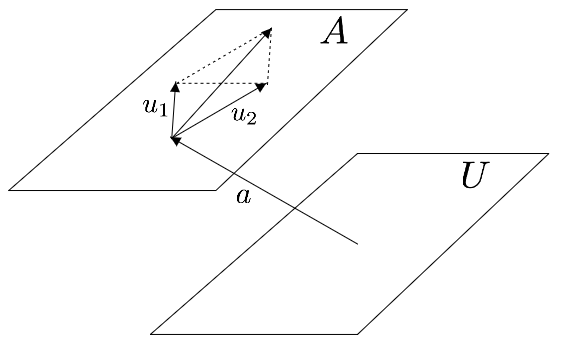
\includegraphics[height=5cm]{./image/3-d-8.png}
    \end{figure}
  \begin{proof}
    If $A$ is an affine subset, i.e., there exists some subspace $U$ and $a\in
    V$ such that $A=a+U$, then for all $\lambda\in\mathbb{F}$ and $v,w\in A$,
    \[
      \lambda v+(1-\lambda)w = \lambda(a+u_1) + (1-\lambda)(a+u_2) = 
      a + (u_1+(1-\lambda)u_2) \in A
    \]
    where $u_1$ and $u_2$ are some elements in $U$. \par
    Now we suppose $\lambda v+(1-\lambda)w\in A$ holds, fix $a\in A$ and let $U=
    \{a_1-a \,:\, a_1\in A\}$. By the hypothesis, for every scalar $\lambda$ and 
    $a_1\in A$, $a + \lambda(a_1-a)\in A$. Therefore, for every $u_1 = a_1-a \in
    U$, $\lambda u_1\in U$. Meanwhile, let $u_2=a_2-a\in U$, $(u_1 +u_2)/2\in U$
    as 
    \[
      a+\frac{1}{2}(u_1+u_2) = a + \frac{1}{2}(a_1+a_2-2a) = 
      \frac{1}{2}a_1+\frac{1}{2}a_2.
    \]
    Hence, by the previous result, $u_1+u_2\in U$. Thus, $U$ is a subspace and 
    $A=a+U$ is an affine subset.
  \end{proof}

  \paragraph{10.}
  \begin{proof}
    Let $A$ be the intersection of every collection of affine subsets of $V$ and
    suppose $A$ is nonempty. Let $v,w\in A$ and $\lambda\in\mathbb{F}$. Then, by
    Exercise 8, for every affine subset $A_{\alpha}$ of $V$, $\lambda v+ (1-
    \lambda)w\in A_\alpha$. Hence it also belongs to $A$. Thus, $A$ is also an
    affine subset of $A$ (as long as nonempty).
  \end{proof}

  \paragraph{12.}
  \begin{proof}
    Let $\{a_1+U,\dots, a_m+U\}$ be a basis of $V/U$ and we first prove a small
    result: for every $v\in V$, there exists an unique list of $v_1,\dots,v_m\in
    \mathbb{F}$ such that $v - (v_1a_1 + \cdots v_ma_m)\in U$. Suppose that 
    $v_1\hp,\dots, v_m\hp$ is such a list as well. Then 
    \[
      (v - (v_1a_1+\cdots+v_ma_m))-(v - (v_1\hp a_1+\cdots+v_m\hp a_m)) \in U.
    \]
    Therefore,
    \[
      (v_1-v_1\hp)a_1+\cdots+(v_m-v_m\hp)a_m \in U = 0+U,
    \]
    Hence $v_i\hp = v_i$ for each $i=1,\dots,m$, completing the proof.\par
    Therefore, for every $v\in V$, denoting $v_1a_i+\cdots+v_ma_m$ as $a_v$, we 
    may define $S$ to be map which maps $v$ to $(v-a_v,a_v+U)$. Now we show that
    $S$ is linear and bijective. For every $u,v\in V$ and scalar $a, b$, 
    \begin{align*}
      aSu + bSv
      &= a(u-a_u,a_u+U) + b(v-a_v,a_v+U)  \\
      &= ((au+bv)-(aa_u+ba_v), (aa_u+ba_v) + U) \\
      &= S(au+bv).
    \end{align*}
    $Su = 0$ iff $(u-a_u,a_u+U) = 0$ iff $u=a_u=0$ and therefore $S$ is 
    injective. Clear that $S$ is surjective. Thus, $S$ is an isomorphism and 
    $V$ is isomorphic to $U\times(V/U)$.
  \end{proof}

  \paragraph{16.}
  \begin{proof}
    Clear that every vector space with dimension $1$ over field $\mathbb{F}$ is
    isomorphic to $\mathbb{F}$. Hence, it suffices to prove there exists 
    $\varphi\in\mathcal{L}(V,V/U)$ such that $\nul\varphi = U$ and the quotient
    map is just the map we want.
  \end{proof}
% end
